

\chapter{Profiling Tools and Techniques}
\label{prof_tools_techniques}
\paragraph*{•}

\hspace{8mm} 

\noindent To measure the boot time of a platform, there exists a wide
variety of profiling tools and techniques which will be covered in
this section.

For optimizing the boot time in linux, we need to find out what operation/component took more
time to complete. For this purpose, some well known techniques are available. Elinux.org
has a listing of various \href{http://elinux.org/Boot_Time}{tools and techniques}.

\section{Bootchart}

Bootchart is a tool for performance analysis and visualization of the
GNU/Linux boot process. Resource utilization and process information are collected
during the boot process and are later rendered in a PNG, SVG or EPS encoded chart.

Shown below is the result from running the same on an Android Tablet
powered by an Intel Atom Cherrytrail family of SoC, with an Ubuntu 14.04 host.

As seen from it, very little information is available from the output.
Bootchart is more suitable to track down userspace.

\begin{figure}[h]
  \centering
    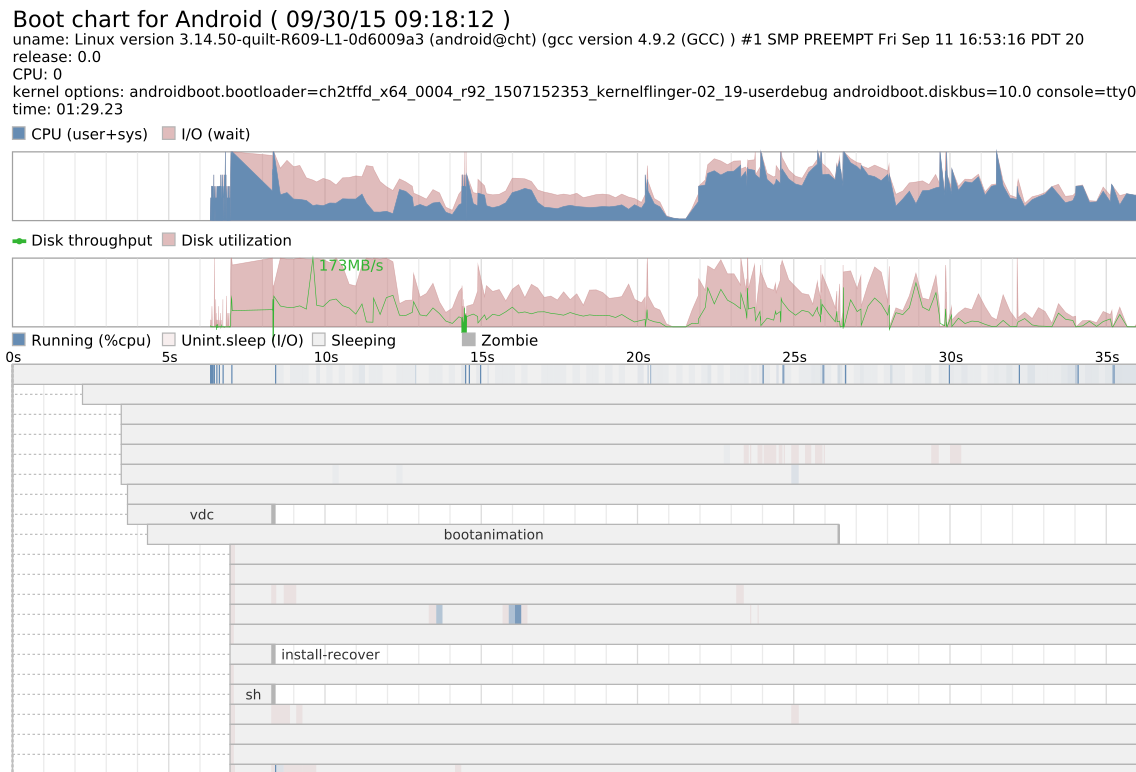
\includegraphics[scale=0.5]{bootchart.png}
    \caption{Bootchart output from Android}
    \label{fig:android_boot}
\end{figure}

\clearpage

\section{Bootloader Timestamps}

Inorder to optimize bootloader, we need to know what operation done by the
bootloader take much of time slice. Even in the debug image, timestamps
are not provided. Hence, we adding timestamp would provide more insight into
the various operations bootloader does. Note that the 
Intel BIOS does not support UEFI Timestamp protocol. There are three
other ways to get the timestamp:

\begin{enumerate}
	\item \textbf{Using UEFI GetTime() function} :
		This is a UEFI Runtime service, and the time is obtained from the CMOS RTC.
		Even though the UEFI supports high accuracy, the CMOS RTC does not support
		resolution lower than 1 second. Hence this method is not suitable.
	\item \textbf{Using Host-side serial timestamp} :
		This method is not an accurate way for getting timestamp.
		However, a resolution of 10 - 50 ms may be obtained.
	\item \textbf{Using RDTSC instruction} :
		Intel architecture from Pentium onwards has the RDTSC instruction
		which returns the number of cycles elapsed since reset. This is so
		far the most accurate way of measuring a timestamp. Below is a
		sample output of the raw cycles read from RDTSC.	
\end{enumerate}

\begin{Verbatim}[fontsize=\small]
4386708900 kernelflinger-02.19-userdebug
4392989550 eMMC storage identified
4397947812 Setting PCI boot device to: Pci(0x10,0x0)/Ctrl(0)/HD
	   (Part1,Sig2568845D-2332-4675-BC39-8FA5A4748D15)
4413724632 oem key size 4096 keystore size 32768
4420869516 Bootlogic: Choosing boot target
4427145072 Bootlogic: Check watchdog\ldots
4433310090 Found RSCI table
-----------------------------------SKIPPED-------------------------------------
5860850202 Loading the ramdisk
5865233400 ramdisk size 5107662
5883670764 Loading the kernel
5908591854 Starting watchdog for 60 seconds
[    0.049605] ENERGY_PERF_BIAS: Set to 'normal', was 'performance'
[    0.049605] ENERGY_PERF_BIAS: View and update with x86_energy_perf_policy(8)
[    0.856330] uart(1) device(INT33A2) wake_src(2) idle(40)
[    0.863966] hpet: number irqs doesn't agree with number of timers
\end{Verbatim}

The more than the ticks, it will make more sense if the value is in the unit of time.
For this, we need to get the TSC clock frequency and calculate the time corresponding
to each of the values. This can be done using an instruction RDMSR. Using this
instruction we can read a specific Model Specific Register which will contain the value
of the TSC clock frequency. Using this value, we can easily calculate the actual time
rather than clock ticks since reset. The below output shows the log from the same
device, showing the time in microseconds since reset:

\begin{Verbatim}[fontsize=\small]
kernelflinger-02.19-userdebug
3298 eMMC storage identified
6045 Setting PCI boot device to: Pci(0x10,0x0)/Ctrl(0)/
     HD(Part1,Sig2568845D-2332-4675-BC39-8FA5A4748D15)
16018 oem key size 4096 keystore size 32768
20322 Bootlogic: Choosing boot target
24017 Bootlogic: Check watchdog\ldots
27688 Found RSCI table
29844 Bootlogic: Check osloader command line\ldots
34511 Bootlogic: Check fastboot sentinel\ldots
38799 checking for force_fastboot
42630 Bootlogic: Check magic key\ldots
-------------------------------SKIP--------------------------------------
951647 Creating command line
954782 wake_source = 0x00
957239 reset_source = 0x01
960518 Loading the ramdisk
963065 ramdisk size 5107662
975021 Loading the kernel
991294 Starting watchdog for 60 seconds
[    0.049633] ENERGY_PERF_BIAS: Set to 'normal', was 'performance'
[    0.049633] ENERGY_PERF_BIAS: View and update with x86_energy_perf_policy(8)
[    0.878356] uart(1) device(INT33A2) wake_src(2) idle(40)
\end{Verbatim}

As we see, the bootloader does its job in 991.2 milliseconds.
Much of its time is spent in tasks which require service from the
firmware, which is outside of the bootloader to control.

\section {Initcall Debug}

This is a method to identify the timings for the init call completions
of the various kernel drivers. This is invoked by changing the kernel
parameters. Simple adding \texttt{initcall\_debug} to the corresponding
BoardConfig.mk would make this change. For achieving this, we need
to make some changes to some scripts, which is a way Intel deals with
multiple configuration for different products they need to support from
the same codebase. Adding \texttt{BOARD\_KERNEL\_CMDLINE += initcall\_debug}
to the corresponding \texttt{BoardConfig.mk} will add it to the default
kernel command line.

Running dmesg will give the log. To get a sorted list, we can use:
\begin{Verbatim}[fontsize=\small]
dmesg -s 128000 | grep ``initcall'' | sed ``s/\(.\)after\(.\)/\2 \1/g'' | sort -n -r
\end{Verbatim}

A sample output of this command in decreasing order of time take to complete would be:

\begin{Verbatim}[fontsize=\smaller]
322342 usecs <7>[    1.230001] initcall i915_init+0x0/0x74 returned 0
254394 usecs <7>[    4.872194] initcall ov8858_init_mod+0x0/0x1000 [ov8858_driver] returned 0
220703 usecs <7>[    0.455998] initcall acpi_init+0x0/0x25e returned 0
214826 usecs <7>[    1.488846] initcall dwc3_pci_driver_init+0x0/0x1b returned 0
209263 usecs <7>[    5.364468] initcall atomisp_init+0x0/0xd51 [atomisp_css2401a0_v21] returned 0
199893 usecs <7>[    0.781643] initcall populate_rootfs+0x0/0xd8 returned 0
133947 usecs <7>[    2.253326] initcall pmic_ccsm_init+0x0/0x14 returned 0
133379 usecs <7>[    5.121348] initcall init_lm3554+0x0/0x1000 [lm3554] returned 0
113899 usecs <7>[    1.890387] initcall intel_pram_init+0x0/0x1d3 returned 0
92015 usecs <7>[    4.975765] initcall init_ov2722+0x0/0x20 [ov2722] returned 0
\end{Verbatim}

\subsection{Total Boot Time}

From the logs obtained above, Bootloader takes 991 milliseconds,
kernel takes 6 seconds, and the userspace takes 18 seconds. The time
BIOS takes is still unknown due to a dependency on BIOS feature for
measuring timestamp and exporting it to kernel through efivars.

